\clearpage
\newpage
\section{Background and state of the art}

\subsection{Faults, Failures and Errors}

During this thesis, the common terminology in fault-tolerant systems \cite{AlgirdasAvizienis2004} is employed:

Any electronic system delivers a service that the user of that system perceives. This service comprises all the external states of the system. A service \textbf{failure} or \textbf{system failure} occurs when the delivered service (i.e., one or more external states) deviates from the correct service state. The correct service is defined by the functional specification of the system. A failure in safety-critical systems can endanger lives or produce high economic losses. Thus, the main goal of safety-critical systems is to minimize the probability of a system failure.

The deviation between the correct internal or external state and the real state is called an \textbf{error}. The cause of an error is called a fault. Thus, a \textbf{fault} is a defect within the system. A fault first causes an error in one of the components that form the system, altering the system's internal state. If this error propagates to the system's output altering the external state and the service provided, we will say that the error led the system to a failure. However, not all faults produce errors and not all the errors reach the external estate of the system producing a failure.  

For instance, consider a two-inputs AND gate inside a system. If one input of the gate is '1' and the other is '0', the expected output will also be '0'. In this scenario, a fault that flips the logic driving the input with value '0' to a '1' will modify the AND gate output to '1', producing an error. However, if a fault flips the other input from '1' to '0', the output will still be '0', the expected value. 

Following the same logic, an AND gate, whose inputs are driven from two registers, one of them with an incorrect value (error), could correct the error preventing it from spreading to other registers and reaching the output of the system.

Faults can be classified into two main categories: \textbf{Systematic faults} that are related in a deterministic way to a certain cause and are avoidable by construction. These faults can be avoided by taking into account possible faults during the first step of the design or by investing enough resources into verification and validation processes. \textbf{Random faults} that occur unpredictably following a probabilistic distribution and are unavoidable. This work focuses on Common Cause Faults (CCF), a particular type of random faults that will be explained later.

\bigskip


\subsection{Safety Related Systems}

Safety-critical systems are those systems that need to work correctly because otherwise, a failure or malfunctioning could jeopardize people's life or health, produce losses in expensive equipment or cause environmental harm. For this reason, these systems must have mechanisms to lower the failure rates until they happen with a negligible likelihood. For instance, in the standards of the aircraft industry, an acceptable failure rate is $10^-9$ accidents per hour \cite{bowen2000ethics}.

Some errors, like systematic errors, can be found and corrected during the development process or mitigated by applying qualitative measures depending on the desired system integrity level SIL. However, random faults could not be avoided and require special mechanisms to prevent these faults from producing a system failure or at least to minimize the likelihood of these happening until a reasonable stent.  

Faults can also be classified into permanent, intermittent and transient faults \cite{constantinescu2003trends}: Permanent faults produce irreversible physical changes to the hardware. Intermittent faults are those faults that appear in irregular intervals. Transient faults occur because of temporary environmental conditions. 

Transient faults are also called soft errors. These faults alter the normal behavior of the system momentaneously. Transient faults produce a loss of data, but they do not produce any physical damage to the circuit. They are random by nature and can appear at any time in some parts of the system, causing a deviation from the expected behavior. Several sources of transient faults exist: neutron and alpha particles, power supply variations and interconnect noise, electromagnetic interference and electrostatic discharge. These sources can affect one or several transistors, momentarily modifying their behavior. Loss of reliability in digital safety-critical systems is produced mainly by transient faults \cite{benso2003fault}. 

According to Moore's Law, the number of transistors that fit in the same area increase by a factor of two every year. The industry has followed this trend for many years, and even though the trend is slowing down, transistors are smaller every year. Increasing the number of transistors in a system also increases the probability of any of them experiencing a soft error. Besides, lower power voltages, higher frequencies and shrinking transistors geometries make them more vulnerable to other sources of faults. For instance, higher frequencies and smaller interconnect features increase the possibility of violating the timing safety margins of the system. Also, lower voltages along with smaller transistors make systems more vulnerable to neutron and alpha particles \cite{constantinescu2003trends}. Hence, this trend has a negative impact on systems reliability. 

Also, with smaller transistors, variations in the manufacturing process (in widths, lengths, oxide thickness, etc.) are more likely to produce systematic failures in the integrated circuits. 

Safety-critical systems must operate correctly even in the presence of faults. The systems that integrate mechanisms to allow a correct operation even when faults appear are called fault-tolerant. Fault-tolerant systems must include two basic mechanisms: fault detection and recovery.

The system must be equipped with components able to detect the errors and prevent them from propagating to other components. When the error is spotted, these components alert the system to trigger a recovery mechanism that puts the system in a previous error-free state.

When the system detects an error, it can recover the last known error-free state, reset the system by powering off or enter a safe state mode, for example, in the event of a permanent fault. However, detecting a transient fault in our system is not always easy. Resetting the system is not always possible and recovering the last error-free state requires a mechanism to store those states. 

\bigskip



\subsection{Redundancy}

Errors are usually detected by employing redundancy. Redundancy is applied differently for different parts of the system. For instance, Error Correction Codes (ECC) is employed to protect the stored data \cite{alcaide2019software}. The data is encoded whit redundant information which allows for detecting errors. In the case of the computing elements, two different kinds of diversity are employed: Time redundancy and space redundancy.

When \textbf{time redundancy} is applied, the same operation (an instruction or a set of instructions) is executed several times (more than once) in the same processing unit. On the other hand, \textbf{space redundancy} is achieved by replicating several times a given processing unit that performs the same operation. This approach is called Dual Modular Redundancy (DMR) \cite{gomaa2003transient}, \cite{lafrieda2007utilizing}, \cite{mukherjee2002detailed} when two core replicas exits on the sytem and Triple Modular Redundancy (TMR) \cite{iturbe2019arm} when the number of replicas is trhee. In a free-error execution, all the outputs must coincide. Therefore, by comparing the different generated outputs, either by the different executions or in the different processing units, the system is capable of detecting possible errors. 

When the different outputs do not coincide, the system has to activate a recovery mechanism to restore the system to a safe state and re-execute from there. This safety state can be a previous free-error state stored in memory or could be achieved by dropping the task if the time constraints allow it. For instance, a system executing a task with a small period (e.g., every 50 ms), such as braking and steering, must perform the task before its Fault Tolerant Time Interval (FTTI) (e.g., 200 ms). In this example, the FTTI is big enough w.r.t the task period to allow the system to drop the task and execute it all over again as long as two consecutive faults do not occur.

Time redundancy is effective against transient faults since it is highly improbable that a transient fault affects two consecutive executions in the same way, and the free-error execution output and the erroneous output will differ, allowing the comparator to detect the error. However, a permanent fault will cause the same error in both executions, making it impossible for the comparator to detect the error. On the other hand, space redundancy is more suitable to effectively detect permanent faults since it is likely that a systematic fault affects only one of the replicas of the hardware. 

Space redundancy has a significant area penalty because of the replication of processing units, but the performance loss is negligible since all the operations are performed in parallel. On the other hand, time redundancy has no area overhead, but the performance degradation is high since the same operation has to be performed several times sequentially.

Redundancy is based on the idea that the probability that all the replicas produce the same error is near zero. This assumption is valid in most of the cases since most of the faults are independent. However, if the same cause is responsible for different faults in the different replicas, faults are not independent anymore and the previous assumption is not valid.

\bigskip


\subsection{Sphere of Replication}
\label{section:SoR}

The Sphere of Replication (SoR) \cite{hernandez2014live}, is the granularity at which the outputs of the replicated elements are compared to detect errors. In Figure \ref{fig:SoR}, extracted from \cite{hernandez2014live}, several granularity levels are illustrated. They range from the finest granularity (a) to the most coarse one (d). Comparing data between pipeline stages as in (a) is not practical due to the enormous hardware and performance overhead required to perform the comparison each cycle. Instruction granularity can be applied as shown in \cite{reinhardt2000transient}, where the authors propose executing redundant threads in a superscalar microprocessor with the capacity to execute several threads in different functional units. However, this approach is not exempt from drawbacks since special communication channels are required to perform the comparison at instruction-level granularity. On the other hand, a finer granularity means faster error detection and faster and easier recovery mechanisms. 

However, most of the approaches used in the industry rely on an off-core-level SoR. In this case, only the data written to the system memory or the I/O interface is compared. This approach takes advantage of the fact that a task finishes without errors when the service provided (state of the I/O and memory) is correct, and provided that the external states are correct, the internal states (e.g., in-core activity) can be ignored. Also, the overhead is much lower than the instruction-level SoR overhead. With off-core-level SoR, only the addresses and values sent by the cores through the communication-network are needed to perform the comparison. Hence, snooping the information flowing through the communication-network is enough and the intrusiveness of this solution is much lower. However, the time elapsed from a fault occurrence and the error detection is unbound. For instance, an error could be confined to the register file during most of the program execution time without reaching the communication-network. This is an issue for safety-critical real-time systems where each task has strong time constraints.

\begin{figure}[h]
    \centering
    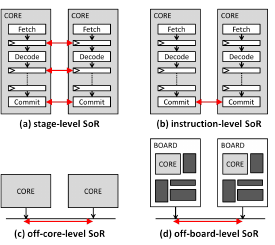
\includegraphics[scale=1.25]{img/differentSoR.png}
    \caption{Figure 2.2: Schematics for different SoR granularities \cite{hernandez2014live}}
    \label{fig:SoR}
\end{figure}
\bigskip





\subsection{Dependent failures and Common Cause Fauilures}
\label{section:CCFs}

Dependent failures \cite{Tummeltshammer2009} are characterized by their occurrence probability. Whereas the occurrence probability of several failure events produced by independent faults can be computed as the product of all their occurrence probabilities, the occurrence probability of dependent failures can not be modeled in the same way. Hence, the following expression applies to two independent failures A and B, but is not valid if failures A and B are dependent. \[P(A) P(B|A) = P(B) P(A|B) = P(A) P(B)\]

Usually, as shown in the expresion below, the probability of two dependent failures is higher than that of two independent failures caused by independent faults. \[P(A) P(B|A) > P(A) P(B)\]

This issue has to be considered since redundancy is based on the assumption that the likelihood of two replicas experiencing the same failure is virtually zero.

CCFs are a type of dependent failures that arise simultaneously in redundant elements from a single shared cause. In safety-critical systems implementing space redundancy, CCFs may produce the same failure in all the replicas. If this happens, the error detection mechanism will fail since both erroneous outputs coincide. For this reason, CCFs are a hazard for safety-critical systems and all fault-tolerant systems standards consider CCFs' effects.

For a CCF to occur, the system must have at least two channels (two replicated elements). A CCF arises when a fault that is the root cause spreads through a coupling mechanism to all the system channels. For instance, suppose a fault-tolerant two-channel system (i.e., two redundant cores in the same die) where the cooling system fails. The root cause is the failure of the cooling system. The heat is not dissipated anymore, and the temperature in the whole die increases. In this example, the thermal coupling becomes the mechanism responsible for the fault cause affecting both channels.

Notice that both systematic and random faults can also cause a CCF. For instance, typical examples are a soft error affecting the clock logic of the two cores or a voltage droop. Defects on the design of the hardware of the replicas or in the manufacturing process (e.g., identical physically low gates in the replicas) could affect all the channels in the same way producing a CCF.

Figure \ref{fig:Coupling_mechanisms} shows the most relevant fault coupling mechanisms \cite{Tummeltshammer2009}, which are described in the following paragraphs. 

\begin{figure}[h]
    \centering
    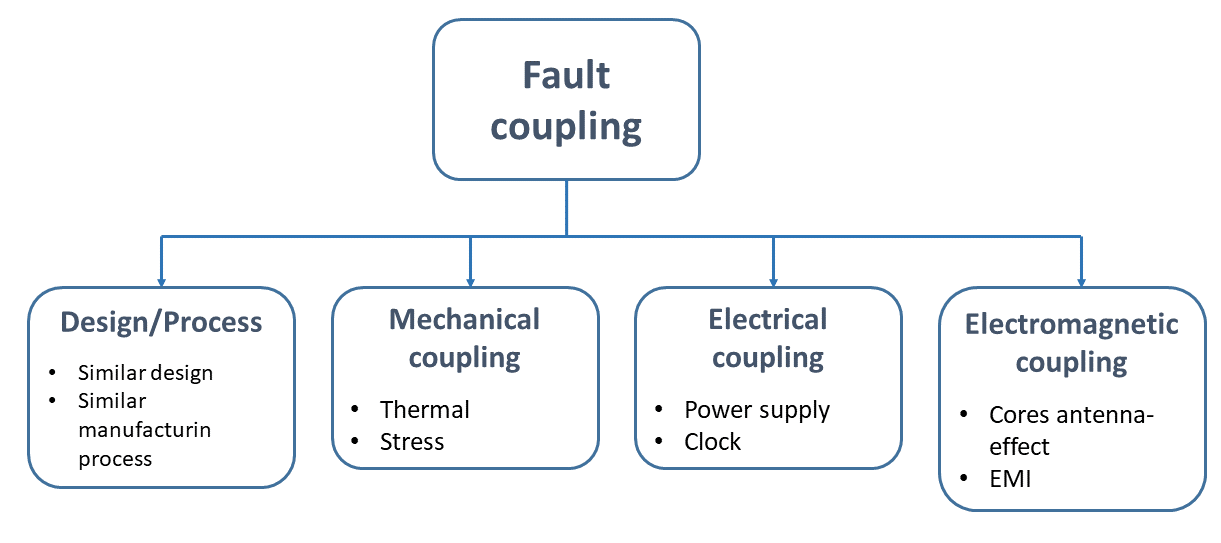
\includegraphics[scale=0.5]{img/Coupling_mechanisms.png}
    \caption{Most relevant fault coupling mechanisms}
    \label{fig:Coupling_mechanisms}
\end{figure}

\textbf{Coupling by similar design or fabrication process:} Usually same software and hardware designs are employed for all of the system channels (e.g., all the cores have the same design and the software they execute is also the same). Employing different hardware or software for each channel will dramatically increase the design and test costs. Hence, a fault in the design or the manufacturing process must be prevented during the design process or detected during the testing. Otherwise, it will be missed by the fault-detection mechanism even if redundancy is applied. 

\textbf{Mechanical and Thermal coupling:} The mechanical and thermal coupling effects are transmitted slowly over the SoC die compared to the processor operation speed. It is assumed that a CCF can only arise if the effects of the mechanical stress or the heating affect the same gate/transistor of all of the replicas at the same time. However, this is very unlikely due to the slow propagation of these physical effects. The most hazardous scenario would consist of a short circuit producing a very focused and abrupt temperature increase. This could result in a CCF if the affected point presents a perfect symmetry w.r.t the affected gates/transistors. It is assumed that mechanical stress affects the whole die, and therefore, it does not represent a CCF risk. 

\textbf{Electromagnetic coupling:} Electromagnetic coupling can affect the layout when the paths of the cores act as an antenna for the electromagnetic field. This could result in voltage changes producing soft errors in both replicas. If the layout of all the replicas is identical, the effect of the electromagnetic fields is very likely to be similar in all the system channels. However, the small dimensions of the VLSI protect them against frequencies below 100GHz, since the circuit paths only work as antennas for higher frequencies. PCB traces are much more vulnerable to electromagnetic fields. Therefore, it is improbable that electromagnetic fields produce a CCF in an integrated circuit.

\textbf{Electrical coupling:} Usually, both cores share the power supply and some signals such as the clock. Therefore, a perturbation in the power supply, e.g., voltage droop or noise or a soft error in the clock logic, can affect all the replicas of the system analogously. Unlike mechanical or thermal coupling, electrical coupling affects the whole system concurrently, and hence, in case of similar effects, a CCF that can not be detected by the comparator unit of the fault detection mechanism will occur. Thus, diversity is not enough to prevent system failures when a fault affects the different replicas in the same way and extra measures must be applied. 

Notice that even though single event upsets (SEUs) caused by particle radiation are one of the major causes of failures in electric systems [14], they usually affect a tiny area (usually a single register or cell RAM), making it very unlikely for them to produce a CCF.   

To protect the system against CCF and comply with the safety standards, the redundant elements in the system must show diversity among them. Thus, diverse redundancy can be achieved in different ways: 

\textbf{Design diversity} consists of achieving hardware procuring the same functionality but implemented in a different way. Design diversity can be achieved at different abstraction levels. For instance, the same functionality can be performed with two different architectures, or the same architecture can be implemented using different gate libraries or different technology. Design diversity is very effective in preventing transient and systematic faults from causing a CCF since it is improbable that any fault affects all the replicas of the system analogously. However, implementing two diverse components is associated with a considerable increase in design costs.

\textbf{Time diversity} is reached by ensuring that the redundant software executions in the replicas are staggered, i.e., the redundant cores are always executing different instructions, and thus their internal states are always different. Being the internal states different, a transient fault affecting all the cores analogously will produce different results and thus, the errors will be detected by the fault-detection mechanism. Applying time diversity implies lower costs and design efforts. However, time diversity is vulnerable against systematic faults that affect all the replicas analogously. %This approach, if realized with two cores, is referred to as Dual Core LockStepping (DCLS) and is used by several commercial processors [15], [35], [37].


\bigskip


\subsection{Lockstep execution}

The lockstep architecture implements two identical processors that perform a staggered execution of the same software (i.e., one core is always some instructions ahead of the other core). Lockstep execution provides a mechanism to detect CCF by implementing diverse redundancy in the system. The next section shows two different approaches for achieving a lockstepped execution.

\subsubsection{Tight hardware-based lockstep execution}

This approach is broadly used. For instance, it is implemented in the Infineon AURIX family \cite{infineon2012aurix}. In a hardware-based lockstep implementation, two identical instances of the same processor are employed (DMR). Figure \ref{fig:HWlockstep} shows a simplified schematic of this approach. Both processors execute the same instructions with a small-time shift of N cycles (usually 2 or 3 cycles). The outputs of both processors are compared by hardware, detecting any possible mismatch between both executions. Also, since both cores have some cycles of staggering by design, the system exhibits time diversity, and hence it is protected against CCFs. 

Both cores assume a different role in this technique. The core that goes ahead in the program execution will be the head core, while the core that is behind in the execution will be the trail core. As shown in Figure \ref{fig:HWlockstep}, the inputs are the same for both cores, although the trail core needs to queue the inputs in a buffer for N cycles. The head core's external requests (data load/store, interrupts, etc.) are stored in a buffer during N cycles until the trail core performs the same requests. Requests of both cores are compared before leaving the core complex. The error is detected in the event of a mismatch, and the proper recovery mechanisms can be applied.

\begin{figure}[h]
    \centering
    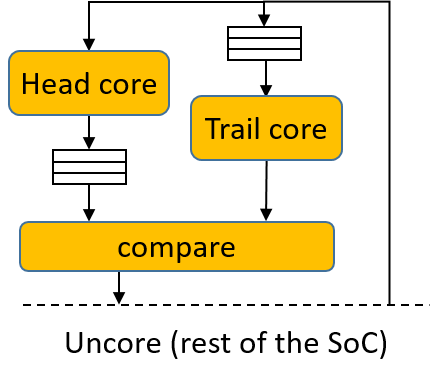
\includegraphics[scale=1]{img/HWlockstep.png}
    \caption{Schematic of the tight hardware-based lockstep}
    \label{fig:HWlockstep}
\end{figure}

As mentioned in section \ref{section:SoR}, errors can only be detected once they leave the core complex and are visible at the outputs. Therefore, any fault can go undetected for an arbitrary number of cycles that depends only on the workload. Some mechanisms can be applied to reduce the error time detection as described in \cite{hernandez2014live}. In this work, a mechanism to periodically send the file registers values through the system communication-network to detect errors before they reach the ouputs of the cores is proposed.

This lockstep implementation hides its complexity to the user, who perceives everything as one single processor, easing the development process. However, for the same reason, performance is halved since both processors can not be used to execute different non-critical tasks that do not require lockstepped execution. At the same time, this approach is very intrusive and significant hardware modifications are required to implement this solution in a couple of cores.

\bigskip


\subsubsection{Light-weight software-based lockstep execution}
\label{section:software_light_lockstep}

This approach is proposed in \cite{alcaide2020software}. The idea is to create diverse redundancy at the software level by running a program twice on different cores. To implement this approach, no hardware modifications are needed. Thus, the intrusiveness of this approach is null in hardware terms and can be implemented with Commerical off-the-shelf (COTS) products.

Light-weight software-based lockstep execution requires three cores: one for monitoring the execution of the critical tasks and ensuring that the minimum required staggering between the redundant executions is maintained, and two identical cores to perform the redundant execution of the critical task. Figure \ref{fig:SWlockstep} shows a simplified schematic of the light-weight software-based lockstep hardware implementation. The monitor core executes the monitor thread, which is in charge of scheduling the redundant processes in the two different cores and periodically obtaining the number of executed instructions by each redundant core ($\#instr$ in Figure \ref{fig:SWlockstep}). The monitor only allows the trail core to make progress if staggering is bigger than a given threshold  ($\#instr_{head} - \#instr_{trail} > TH_{stag}$). This condition is checked by the monitor every $T_{check}$ cycles. $TH_{stag}$ and $T_{check}$ have to be selected such as if the trail core executes in $T_{check}$ the maximum possible number of instructions while the head core is stalled, the staggering still is bigger than zero. Only when the head core finishes the execution of the critical task the monitor allows the trail core to run without exercising any control over it. 

The monitor thread is in charge of keeping a proper staggering between both redundant executions to procure time diversity. However, the monitor does not provide a mechanism to detect faults during the execution. This checking mechanism is implemented by software means and when the execution finishes, its results are compared between cores.

The core executing the monitor thread is unprotected against CCFs. Therefore, its execution requires a hardware-based lockstepping. The thread monitor is also in charge of handling the inputs and the outputs of the system. Two input readings from both redundant processors at different times could result in different read values, which would make the execution results differ.  

This approach achieves a lockstepped execution with null intrusiveness in hardware terms. However, there is a trade-off between the period $T_{check}$ and the minimum staggering allowed $TH_{stag}$. The smaller the $T_{check}$ period, the more significant the thread monitor computational overhead. Also, the smaller $T_{check}$ period is, the trail core can execute fewer instructions in that period, and the $TH_{stag}$ is smaller. This trade-off is usually resolved by choosing a staggering equal to the number of instructions the core can execute in 100$\mu$s. Therefore, the biggest drawback of this approach is its high staggering.

Note that with the light-weight approach, both cores can execute the same redundant tasks when the criticality level is high, ensuring a safe execution or two different non-critical tasks when lockstepped execution is not required. In the last case, the light-weight approach doubles the performance.

\begin{figure}[h]
    \centering
    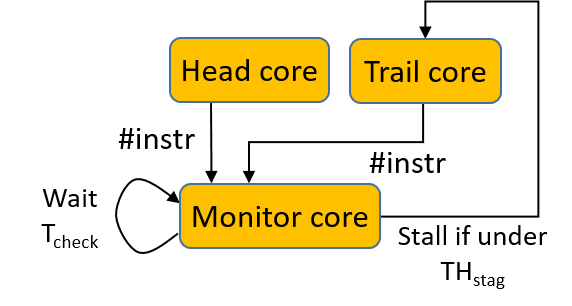
\includegraphics[scale=1]{img/SWlockstep.png}
    \caption{Schematic of the light-weight software-based lockstep}
    \label{fig:SWlockstep}
\end{figure}

\bigskip


%\subsection{Triple Modular Redundancy???}
